In living cells, processes are regulated by networks of interacting molecules.
Aberrations in these networks underlie a wide range of pathologies. The development of new therapies
requires obtaining a thorough insight in the functioning of these networks, which is a challenging task.
Feedback loops and crosstalk between pathways lead to an intricate wiring of the network.
Hence, it is necessary to study the ensemble of molecules involved, because the 
behavior of individual molecules is not sufficient for a complete understanding. 
Since the human brain is ill-suited to grasp the non-linear dynamics of these complex networks and
the entailed emergent properties, computational support has a growing role 
in molecular biology.

The systems biology approach to understanding biological systems starts off from a
scientific question and then follows an empirical cycle \--\ or rather a positive spiral \--\ of
knowledge/theory $\rightarrow$ model $\rightarrow$ hypotheses $\rightarrow$ experiments $\rightarrow$
observations $\rightarrow$ update and/or refinement of knowledge/theory,
until an answer to the original question is found (Figure~\ref{fig:empirical-spiral}).
A model plays a pivotal role in this cycle:
\begin{enumerate}
  \item to organize data and store knowledge,
  \item to structure reasoning and discussion
  \item to perform \emph{in silico} experiments and derive hypotheses.
\end{enumerate}
An \emph{in silico} model is always a simplified representation of biological reality and is never the 
aim in itself.
Rather, it is a powerful means in the process of gaining an understanding of the biological system.
Given its role in the empirical cycle, the process of modelling is especially effective
when applied by the experts with respect to a certain biological system. Biologists usually have a good sense 
of cause-and-effect relationships of molecular interactions. In addition, they are the most knowledgeable
on the network topology and the dynamics of the biological system they are studying.
Since they also benefit most from the generation of hypotheses and from an efficient experimental design, 
biologists would be the primary candidates to construct models of their research topic.

\begin{figure}[!htb]
  \centering
  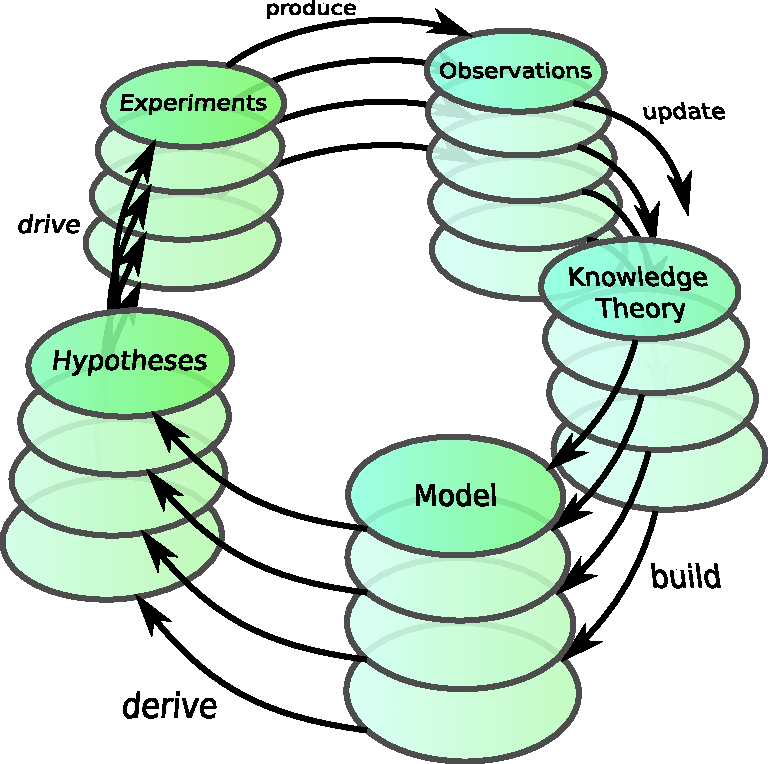
\includegraphics[width=0.35\textwidth]{images/empirical_spiral4}
 \caption{The empirical spiral.}\label{fig:empirical-spiral}
\end{figure}


As models are a formalization of knowledge or theories, an underlying formalism is needed to express
this knowledge. Different formal methods have been successfully applied to construct representations
of biological systems. Among these methods are Boolean logic~\citep{boolean-networks-flower,boolean-networks2},
ordinary differential equations (ODEs, reviewed by~\citealp[]{hidde-review}),
interacting state machines~\citep{interacting-sm1,interacting-sm2},
process calculi~\citep{blenx,bio-pepa}, Timed Automata~\citep{ta-siebert,bartocci-oscillators,
oded-ode-ta-discretization} and Petri nets~\citep{petri-nets,petri-nets2}.
Most of these formal methods have been implemented into software tools to aid the process
of modelling. Due to the lack of such a supporting tool, \tas\ have remained a less 
frequently applied method.

\cite{ta-siebert} use \tas to extend a classical modeling paradigm
~\citep{thomas-formalism}, allowing to add temporal dynamics to gene network models.
\cite{bartocci-oscillators} describe a model of biological oscillators and test 
synchronization properties in this dynamic system.
A discretization of ODEs to \tas\ is proposed by~\citet{oded-ode-ta-discretization}, applying
this translation between the two formalisms to an example gene regulatory network. Two 
different approaches to transforming
a Petri net model into \tas\ are presented by~\citet{ta-giapponesi},
who also address the important issue of state space explosion in their paper.
Finally, \cite{ta-radiazioni} propose an \emph{ad hoc} \tas\ model of a radiation treatment
system, which is then validated through UPPAAL.\\
Each of these approaches has been successfully validated and demonstrates the power of \tas,
both on the theoretical level and in real biological applications. However, none of the listed approaches
has led to a tool implementation of the proposed method, the application of which was often limited to simple
or specific examples. The challenges of a broader applicability of \tas\ were not previously considered,
nor was the usability of the approach evaluated from the point of view of a biologist.

However, mastery of these tools requires
training and experience in mathematical modelling. In this respect, a lack of tradition in quantitative
reasoning and formal methods within the biological community at large is still a stumbling block for
widespread application of modelling of biological systems. Here, we present an intuitive method for the
construction of formal in silico models of the dynamics of molecular networks, supported by a novel,
user friendly modelling tool, ANIMO (Analysis of Networks with Interactive MOdeling,~\citealp[]{animo-bibe}).

In the Methods section, we will explain how choosing a suitable abstraction level can make the construction
of models more intuitive. We will then show how ANIMO is designed to support the modelling process following
this approach. Construction of a small model based on experimental data will exemplify the method that we
propose. In the Results section, we first show an ANIMO model of the genes and proteins that constitute
the circadian clock network in Drosophila Melanogaster. The remainder of that section is dedicated to
illustrate how a single modelling iteration in the empirical cycle is used to compile prior knowledge and
experimental data into a model and derive meaningful biological hypotheses from this model. These hypotheses
find ample support in literature.
